\chapter{シェル}

\section*{システムを包み込むシェル}

「シェル(shell)」とは、英語で「貝殻」のことを言う。
昭和シェル石油のマークは、貝殻がモチーフになっているが、
これは英語で考えるととてもわかりやすい。

ところで、今回紹介するシェルとは、 UNIX システムのコアの部分を包み込み、
ユーザとシステムの仲介役をしているしくみのことだ。
シェルは、 UNIX システムでコマンドの入力を手助けしてくれる。
シェルにはとても強力な機能が備わっていて、これを使いこなせれば、
 UNIX システムを少ない入力で、これまでの何倍も活用することができる。

\section{ユーザ・インターフェース}

 UNIX システムは、基本的にコマンドをキーボードから打ち込む
コマンド・ラインをベースにしたユーザ・インタフェース
\footnote{user interface: ユーザがシステムを使うときに相手にする部分}
を採用している。
一方、 MacOS や Windows は、アイコンをマウスで操作する GUI\footnote{Graphical
User Interface: グラフィカル・ユーザ・インタフェース} をベースにした
システムだ。

シェルは、コマンド・ライン・ベースのインタフェースを使うときに、
ユーザをサポートする。
その役割をはっきりさせるために、コマンド・ライン・ベースのインタフェースと
 GUI の話を最初にしよう。

コマンド・ライン・ベースと GUI、この 2 種類のインタフェースには、
それぞれ特徴がある。

\subsection{GUI の特徴}

まず GUI の方は、絵の描かれたカードを持って、
コンピュータとお話をしているというイメージを持ってもらえばいいだろう。

例えば、 WWW にアクセスするときには、 Web ブラウザの描かれたカードを
持ってコンピュータに見せる。
すると、コンピュータが Web ブラウザを起動してくれるというわけだ。

このシステムには、絵が描かれたカードが最初から用意されていて、
はじめてコンピュータを使う人にも、「なんとなく」使い方がわかり、
とっときやすい。
このシステムは、ブラウザとか、お絵描きソフトとか、
ゲームなどを単に起動して使うときにはとても便利だ。

\subsection{コマンド・ライン・ベースのインタフェースの特徴}

一方、コマンド・ライン・ベースのシステムの方は、文字を書いて
コンピュータとやりとりをしているようなイメージになる。

つまり、例えば WWW にアクセスするには「netscape」とかいう文字を書いて、
コンピュータに指示を出し、 Web ブラウザを起動してもらう。
このコンピュータに指示をするときに使う言葉が、コマンドである。
このシステムでは、言葉(コマンド)を知らないと、コンピュータと全くお話
できないため、最初に少し勉強する必要がある。
また、文字を一々書かなければならないので、単にブラウザや、
お絵描きソフト、ゲームなどを起動するにも、たくさんタイプしなければならない。

\begin{figure}[H]
\centering{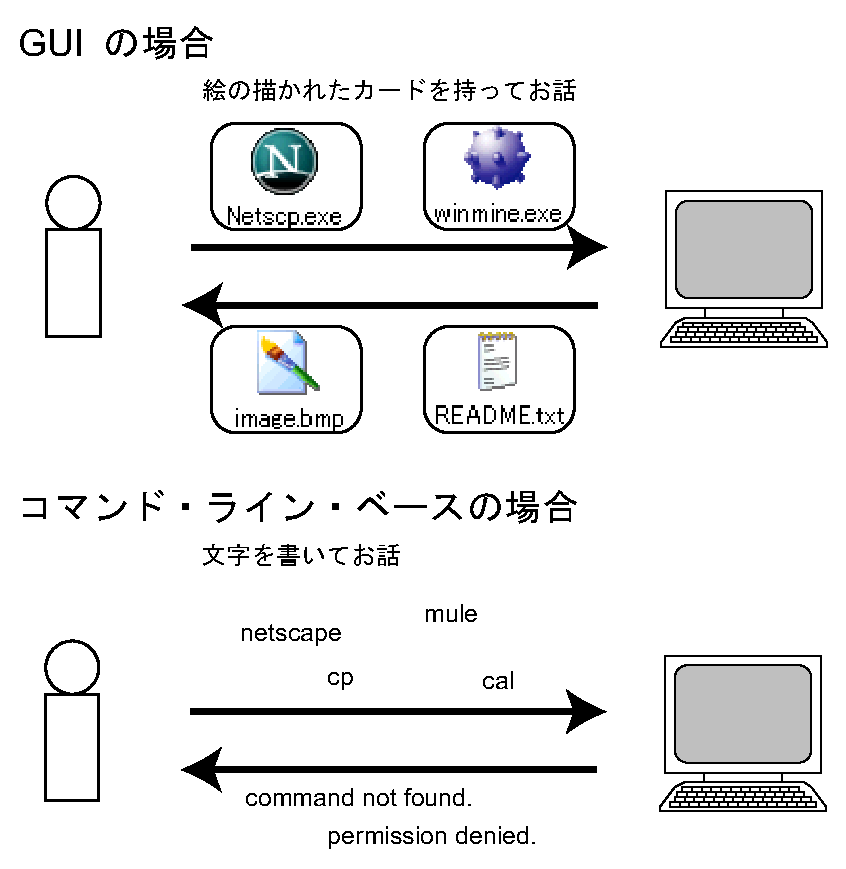
\includegraphics[scale=0.8]{guicui.eps}}
\end{figure}

\subsection{GUI の欠点}

こう書いてくると、 GUI の方が便利そうだが、本当にそうなのだろうか?

\bigskip

 GUI にも問題はある。
まず、コンピュータに細かい指示を出すには向いていないことだ。

例えば、ある箱(フォルダ)にファイルが入っているとしよう。
このファイルを持って、別の箱に突っ込んだら、コンピュータはどう判断するだろうか？~~
ファイルの移動？~~それともコピー？~~

実際 Windows では、同じドライブ間で実行した場合と、
別なドライブ間で実行した場合で、異なった判断をコンピュータがする
\footnote{同じドライブにあるフォルダ間で実行すると、コンピュータは
「移動」を実行する。
別のドライブであれば、「コピー」を実行する。}。
また、それが通常のファイルの場合と、実行型ファイル
の場合でも異なる\footnote{Windows のバージョンによっては、
通常のファイルと異なり、実行型のファイルで
この作業を行なうと、コンピュータはショートカットを作るだけである。}ことがある。
しかも、これらの挙動は、同じ Windows でもバージョンによって異なっていたり
することがあるのである。

\begin{figure}[H]
\centering{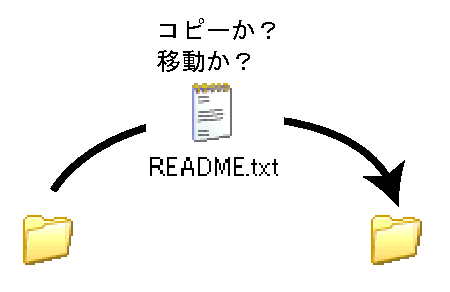
\includegraphics[scale=0.8]{cpmv.eps}}
\end{figure}

また GUI は、抽象的な指示を出すのには向いていない。
例えば、「\texttt{data001}」〜「\texttt{data100}」という 100 個の
ディレクトリ(フォルダ)を作る必要があったとしよう。
 Windows で GUI のみを使う場合、右クリックで \texttt{[新規作成] → [フォルダ]} を実行し、
フォルダの名前(「\texttt{data001}」〜「\texttt{data100}」)を指定するという
作業を 100 回実行しなければならない。

また GUI は、いくつかの連続した作業を一括して自動化するのにも
向いていないのである
\footnote{最近のバージョンの Windows では GUI のツールを
自動化してコントロールするために WSH(Windows Scripting Host)のような
しくみが使えるようになってきている}。

\subsection{コマンド・ライン・ベースの欠点を補完するシェル}

コマンド・ライン・ベースの欠点は、基本的にはたくさんタイプする必要があることだ。
 UNIX システムのシェルは、この欠点を補完する。
シェルは、過去に打ったコマンドを覚えておいたり、同じような繰り返しの作業を
簡単な指定で何百回も実行させたり、いくつかのコマンドをまとめて自動化
する機能を持っている。
この機能を活用すると、ユーザは少ない入力で、さまざまなことを実行できる。
\newpage

\section{シェルの役割}

シェルは、 UNIX システムのコアの部分を包み込んでいる。
ユーザと UNIX システムの間にシェルがある。
ユーザが UNIX システムを使うときに、相手をしているのは、
実は全部シェルなのだ。

\bigskip

ここまで、読んできて、「は？」と思うかもしれない。
「え？ シェルなんて今日の今日まで知らなかったぞ。
一体、いつそんなもの相手にしたっけ？」と思うかもしれない。

ところが、実は UNIX システムでコマンドを打つと、
シェルが一回受け取って、シェルがシステムに渡してから実行されているのだ
(ユーザの知らないうちに)。

\begin{figure}[H]
\centering{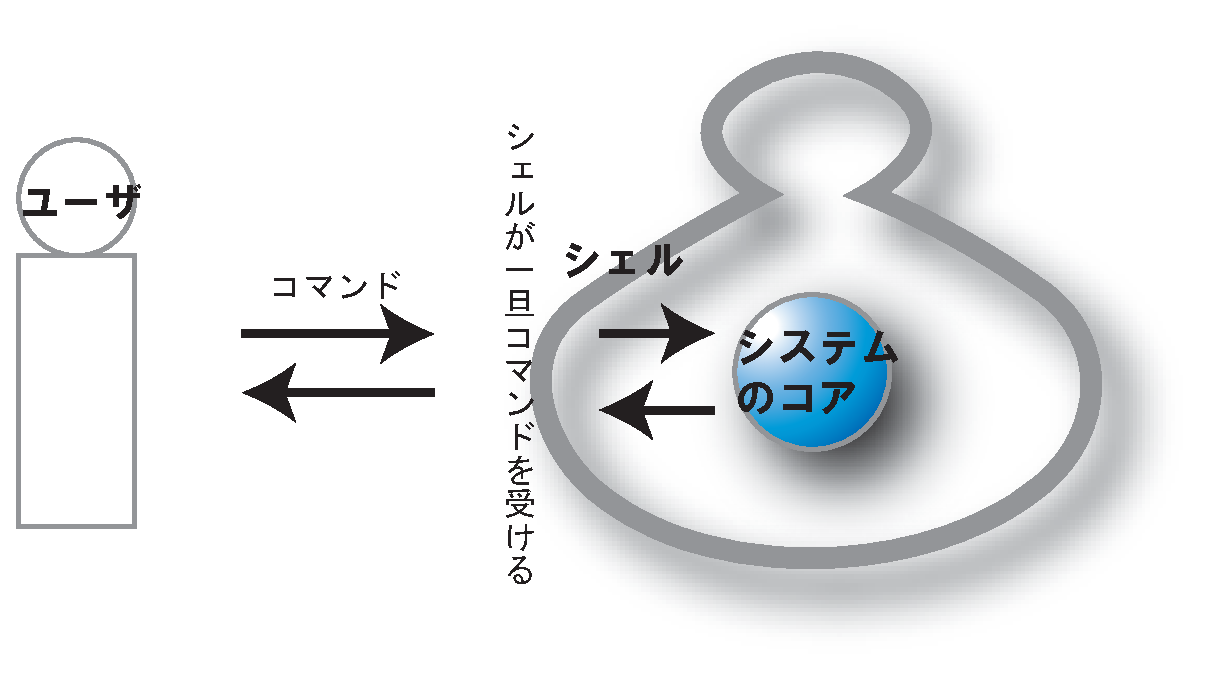
\includegraphics[scale=0.4]{intershell.eps}}
\end{figure}

なぜ、そんな余計なものが間に入っているのだろう？

\bigskip

例えば、「自分好みにシステムを改造したい」と、そう思ったことはないだろか？

そんなとき、コマンドをダイレクトにシステムに渡すように設計されていたら、
システムそのものを改造しなければならない。
ユーザとシステムの間にシェルでワン・クッション入れておけば、
システムを直接改造しなくても、シェルの方をいじるだけでいろいろ自分好みに
カスタマイズすることができるのである。

また、間にシェルが入っていてくれることで、
システムの方には単純なコマンドだけを用意しておいて、
ユーザ相手の部分はシェルがていねいに面倒を見るということも
可能になる。

要するに\underline{システムは単純に、後はシェルにおまかせ}
というコンセプトである。

\begin{figure}[H]
\centering{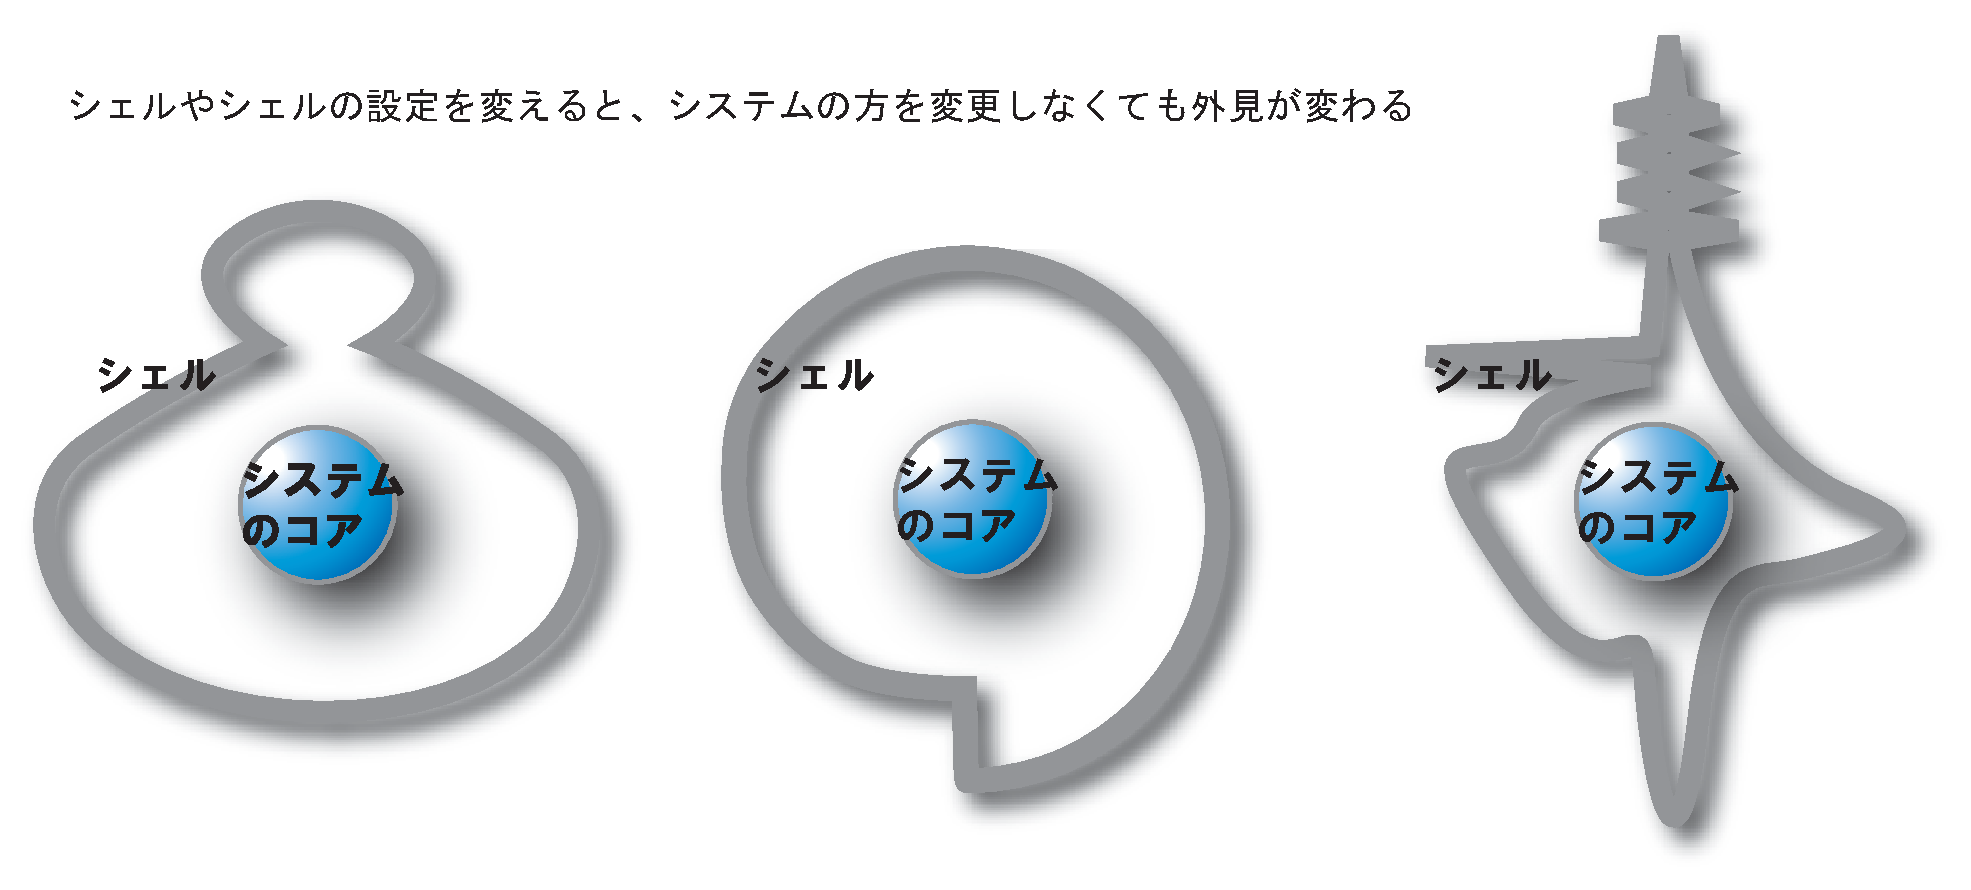
\includegraphics[scale=0.4]{shellchange.eps}}
\end{figure}

\section{いろいろなシェル}

では、シェルを紹介しよう。

代表的なシェルには sh、csh、tcsh、 ksh、 bash、 zsh などがある。

これらを一時的に使ってみた場合には、
単に「\texttt{sh}」とか「\texttt{csh}」と打てばいい。
なお、デフォルトでは「tcsh」になっている。

それぞれ簡単に紹介しておこう。

\begin{list}{}{
\setlength{\leftmargin}{1.5cm}
\setlength{\listparindent}{0cm}
\setlength{\itemindent}{0cm}
\setlength{\labelsep}{0.5cm}
\setlength{\labelwidth}{1cm}
}
\renewcommand{\makelabel}{\large\bf}
\item[sh] 一番単純なシェル。
ボーン(Borune)さんが作ったので、ボーン・シェルとも言う。
\item[csh] BSD のビル・ジョイくんが作った、
 C 言語に似たプログラム機能を持ったシェル。
\item[tcsh] TENEX というシステムにあった、補完機能などを組み込んだ、
csh の機能拡張版。
ただし、 FreeBSD の場合、 csh と tcsh は同じになっている。
\item[ksh] コーン(Korn)さんの作った sh の機能拡張版で、
 AT \& T 社の製品。
ただし、 ksh 互換のフリー・ソフトも作られていて、 FreeBSD には
そちらが入っている。
\item[bash] GNU のソフトでボーン・アゲイン(再び)・シェルという。
 sh の機能拡張版で、 tcsh などの機能も取り入れている。
\item[zsh] 作者曰く、究極のシェル。
sh と csh の機能を取り入れ、独自のプログラム機能を持っている。
\end{list}

\newpage

\section{シェルの機能}

\subsection{ヒストリー機能}

シェルの代表的な機能の一つがヒストリー機能である。
これは要するに、昔打ったコマンドを、システムが覚えていて、
それを後から使えるということだ。

\bigskip

では、具体的に使ってみよう。

まず、シェルにコマンドを覚えさせてみよう。
\texttt{who} 、 \texttt{ls} 、 \texttt{cal} 、 \texttt{ps} などと
 4 つくらいコマンドを実行してみよう。
ここまで打ったコマンドのリストは記憶されていて「\texttt{history}」
と打つと表示される。
なお、システムの設定により、過去 100 個分を記憶しているため、
非常に長い出力がでる。

\begin{progls}
% \slbfl{history}
 [中略]
   101  11:23   who
   102  11:23   ls
   103  11:23   cal
   104  11:24   ps
   105  11:25   history
%
\end{progls}

この表示は、最初が「何番目」のコマンドか、次が実行したのが「何時」か、
最後が「どんなコマンド」を実行したのかを表している。
過去 100 個分を記憶しているために、
ここでは login して最初に実行した \texttt{who} が 101 番目と表示されている。

\subsubsection{\texttt{!「数字」}: 「数字」番目のコマンド呼び出し}

シェルが記憶しているコマンドは簡単に呼び出せる。
例えば、 101 番目の \texttt{w} をもう一度実行するには「\texttt{!101}」と
入力すればいい。
全く同様に、 103 番目の \texttt{cal} なら「\texttt{!103}」である。

では、試してみよう。

\begin{progls}
% \slbfl{!101}
who
ei00000  ttyp0    11/01 01:06   (:0.0)
% \slbfl{!103}
cal
     11月 2000
日 月 火 水 木 金 土
          1  2  3  4
 5  6  7  8  9 10 11
12 13 14 15 16 17 18
19 20 21 22 23 24 25
26 27 28 29 30

%
\end{progls}

このようにとても簡単である。

\subsubsection{\texttt{!「文字」}: もっとも最近打った「文字」で始まるコマンド呼び出し}

ヒストリーには、別な呼び出し方もある。
一番最近打った、「\texttt{c}」で始まるコマンドは、
この例では　\texttt{cal} だが、
これを呼ぶには「\texttt{!c}」と入力すればよい。
もちろん、 \texttt{history} を呼ぶには単に「\texttt{!h}」である。

では、実行してみよう。

\begin{progls}
% \slbfl{!c}
cal
     11月 2000
日 月 火 水 木 金 土
          1  2  3  4
 5  6  7  8  9 10 11
12 13 14 15 16 17 18
19 20 21 22 23 24 25
26 27 28 29 30

%
\end{progls}

なお、これらの機能は、プログラム書いて、コンパイルするときに使うと便利だ。
つまり、コンパイルするには「\texttt{cc -o 「実行型ファイル名」 「コンパイルするファイル名」}」だが、
これは一度実行してしまえば、
コンパイルしなおすには、単に「\texttt{!c}」で済んでしまうというわけだ。

\subsubsection{\texttt{!!}: 直前のコマンドのくり返し}

また、直前のコマンドをくり返すこともできて、それは単に「\texttt{!!}」と
入力すればよい。

たとえば、直前に \texttt{cal} を実行していれば、
「\texttt{!!}」で \texttt{cal} が実行される。

\begin{progls}
% \slbfl{!!}
cal
     11月 2000
日 月 火 水 木 金 土
          1  2  3  4
 5  6  7  8  9 10 11
12 13 14 15 16 17 18
19 20 21 22 23 24 25
26 27 28 29 30

%
\end{progls}

\newpage

\subsection{コマンド・ライン編集機能}

tcsh などの場合、次のような機能もある。

まず、\KEYTOP{↑} (または Mule と同様に \texttt{C-p}) を押していくと、
一つずつ前のコマンドを呼び出すことができる。
また、行き過ぎた場合、\KEYTOP{↓} (\texttt{C-n}) で一つ進むことができる。

更に、呼び出したコマンドは、\KEYTOP{←}(\texttt{C-b}) や、
\KEYTOP{→}(\texttt{C-f}) や、 \KEYTOP{Delete} などを使って、
書き直すことができる。

これらをコマンド・ライン編集機能という。

\subsection{コマンド別名}

csh 以降に作られたシェルには、
たいていコマンドに別名を付ける機能がついている。
このような機能のことを、「エイリアス -- alias」という。

例えば、単に「\texttt{ls}」と打つと、ディレクトリもファイルも
同じように見えてしまう。
そして、ディレクトリの後ろに「\verb+/+」を付けたり、実行型ファイルの
後ろに「\verb+*+」を付けてて表示させるには、
「\texttt{ls -F}」と打てばいいことは既に紹介した。

しかし、それを毎回打つのは面倒である。
そこで、エイリアス機能を使うと、「\texttt{ls}」と打っただけでも、
「\texttt{ls -F}」と打った場合と同じことをするように設定できる。

具体的には「\texttt{alias ls 'ls -F'}」としてやる。
これで「\texttt{ls}」と打つと、「\texttt{ls -F}」が実行されるようになる。
なお、このように設定したエイリアスは、そのシェルを終了するまで有効である。
これを毎回使いたい場合には、後ろの方で紹介するようにシェルの初期設定
ファイルに記述しておけばよい。

では、実際にやってみよう。
まず、「\texttt{ls}」と打ってみよう。

\begin{progls}
% \slbfl{ls}
2000nen         Circle.java     circle.pl       kongetsu        renshuu2
2001nen         circle          circle.py       kotoshi         tanjoubi
2002nen         circle.bas      circle.rb       prog            thismonth
3years          circle.c        hello           renshuu1
4gatsu          circle.f        hello.c         renshuu1.ps
Circle.class    circle.p        hello.c~        renshuu1~
%
\end{progls}

これでは、ディレクトリと普通のファイルの区別は全くつかない。
かといって、毎回「\texttt{ls -F}」と打つのも面倒である。
そこで、エイリアス機能を使う。

\begin{progls}
% \slbfl{alias ls 'ls -F'}
%
\end{progls}

\newpage

では、「\texttt{ls}」と打ってみよう。

\begin{progls}
% \slbfl{ls}
2000nen         Circle.java     circle.pl*      kongetsu        renshuu2
2001nen         circle*         circle.py*      kotoshi         tanjoubi
2002nen         circle.bas      circle.rb*      prog/           thismonth
3years          circle.c        hello*          renshuu1
4gatsu          circle.f        hello.c         renshuu1.ps
Circle.class    circle.p        hello.c~        renshuu1~
%
\end{progls}

確かに「\texttt{ls -F}」と入力した場合と同じになる。

\bigskip

エイリアス機能は、長いコマンドを打つのが面倒なときに使ったり、
上の例のように、毎回使うオプションをはぶいたりするのに使うと便利である。

\bigskip

実は、「\texttt{alias cp rm}」といったアブナイこと
\footnote{こうすると、「\texttt{cp}」と打っても
「\texttt{rm}」になってしまう。}
も、できてしまうので、使うときは注意しよう。

\subsection{名前の補完}

tcsh などの特徴に、ファイル名やコマンドの補完機能がある。
これは、該当するファイルやコマンドが 1 つしかない場合、
 \KEYTOP{Tab} を押すと補完してくれる機能である。

この機能は、口で説明するよりは、やってみた方が早いので、実際にやってみよう。

まず、「\texttt{ls}」と入力してみよう。

\begin{progls}
% \slbfl{ls}
2000nen         Circle.java     circle.pl*      kongetsu        renshuu2
2001nen         circle*         circle.py*      kotoshi         tanjoubi
2002nen         circle.bas      circle.rb*      prog/           thismonth
3years          circle.c        hello*          renshuu1
4gatsu          circle.f        hello.c         renshuu1.ps
Circle.class    circle.p        hello.c~        renshuu1~
%
\end{progls}

この中で、「\texttt{p}」で始まるのは、
「\texttt{prog}」というディレクトリしかない。
この場合、 \texttt{cd} で「\texttt{prog}」の中に移動するには、
「\texttt{cd prog}」と入力すればよいのだが、
このコマンドを全部打つ必要はない。

まず、「\texttt{cd p}」と打つ。

\begin{progls}
% \slbfl{cd p}
\end{progls}

ここで、 \KEYTOP{Tab} を押すと、「\texttt{p}」で始まるファイルやディレクトリは
「\texttt{prog}」の他にないので、次のように名前が補完される。

\begin{progls}
% \slbfl{cd prog}
\end{progls}

また、上の例では、「\texttt{c}」で始まるファイルは 
「\texttt{circle}」〜「\texttt{circle.rb}」まで 8 個ある。
このとき Mule で「\texttt{circle.c}」を編集したければ、
「\texttt{mule c}」まで入力し、\KEYTOP{Tab} を押してあげると、
「\texttt{mule circle}」まで補完される。
その後、「\texttt{.c \&}」だけを補えば「\texttt{mule circle.c \&}」
となり、入力の手間がはぶける。

\section{シェル・スクリプト}

シェルには、いくつかのコマンドをまとめて自動する機能がある。
シェル・スクリプトという簡単なプログラムを書いて、実際に実行してみよう。

まず、次のように「\texttt{test1}」というファイルを Mule で作る。

\begin{progls}
% \slbfl{mule test1 \&}
%
\end{progls}

\texttt{test1} の中身には、次のように書いて、セーブして Mule を終了する。

\begin{progls2}{test1}
ls -F
cal
\end{progls2}

次に「\texttt{test1}」のパーミッションを、
実行可能に変更してみよう。

\begin{progls}
% \slbfl{chmod 755 test1}
%
\end{progls}

すると、この「\texttt{test1}」は、なんと普通のコマンドのように実行可能になり、
中に書いたコマンドをそのまま実行してくれる。

\begin{progls}
% \slbfl{./test1}
2000nen         Circle.java     circle.pl*      kongetsu        renshuu2
2001nen         circle*         circle.py*      kotoshi         tanjoubi
2002nen         circle.bas      circle.rb*      prog/           test1*
3years          circle.c        hello*          renshuu1        thismonth
4gatsu          circle.f        hello.c         renshuu1.ps
Circle.class    circle.p        hello.c~        renshuu1~
     11月 2000
日 月 火 水 木 金 土
          1  2  3  4
 5  6  7  8  9 10 11
12 13 14 15 16 17 18
19 20 21 22 23 24 25
26 27 28 29 30

%
\end{progls}

このような簡単なプログラムをシェル・スクリプトと呼ぶ。
これを使うと、いくつかのコマンドをまとめて一気に実行できる。

また、ここでは触れないが、条件分岐や、ループなどを使った高度な
プログラムもシェル・スクリプト中では行なうことも可能である。

\section{ワイルドカード}

シェルではいつくかの記号が特別の意味を持っている。
今回は、その内のワイルドカードと呼ばれているものを紹介しよう。

ワイルドカードは、似たような名前のファイルを、コマンド一発で何か同じ
処理をしたいときによく使う。

たとえば、\texttt{「I」、「my」、「me」、「mine」、「the」、
「this」、「these」、「those」、「who」、「which」、「when」}
というファイルがあったとしよう。

このとき、代表的なワイルドカードを使うとどうなるか紹介しよう。

\begin{list}{}{
\setlength{\leftmargin}{1.5cm}
\setlength{\listparindent}{0cm}
\setlength{\itemindent}{0cm}
\setlength{\labelsep}{0.5cm}
\setlength{\labelwidth}{1cm}
}
\renewcommand{\makelabel}{\Large\tt}
\item[「\texttt{*}」] \textbf{0 文字以上\footnote{つまり 0 文字でもいい}のさまざまな文字を表す}

例えば「\texttt{th*}」と書くと「\texttt{the}」、
「\texttt{this}」、「\texttt{these}」、「\texttt{those}」のような、
「\texttt{th}」で始まるすべてのファイルにマッチする。
もしも、「\texttt{th}」というファイルがあれば、それにもマッチする。

また、「\texttt{*e}」と書くと、「\texttt{e}」で終わる「\texttt{me}」、
「\texttt{mine}」、「\texttt{the}」、「\texttt{these}」、「\texttt{those}」
にマッチする。

同様に「\texttt{t*e}」と書くと、「\texttt{the}」、「\texttt{these}」、「\texttt{those}」
にマッチする。

更に単に「\texttt{*}」と書くと、すべてのファイルにマッチする。

\item[「\texttt{?}」] \textbf{何か 1 文字を表す}

例えば「\texttt{m?}」なら、 最初が「\texttt{m}」で、次に何か 1 文字だけある
ファイルということで、
「\texttt{my}」と「\texttt{me}」にマッチする。

また、「\texttt{th?se}」なら、「\texttt{these}」と「\texttt{those}」にマッチする。
\end{list}

これらのワイルドカードを使うと複数のファイルを一気に処理できる。

\bigskip

例えば、「\texttt{cat th*}」と打てば、
「\texttt{cat the this these those}」と打ったのと同じことになる。

また、「\texttt{*}」は、一気にファイルを消すのによく使う。
例えば、「\texttt{rm th*}」と打てば、
\texttt{「the」、「this」、「these」、「those」} を一気に消すことができる。

また Mule は「\verb+~+」の付いたバックアップ・ファイルを作成するが、
これを全部消すには「\texttt{rm *\~}」と打てばよい。
なお、間違って「\texttt{rm *}」とすると全部のファイルが消えてしまうので、
注意しよう。

\section{シェルの初期設定をカスタマイズ}

tcsh や csh の初期設定ファイルは、「\texttt{.cshrc}」である。
この中をいじると、シェルの初期設定を変えることができる。
これらの「\texttt{.}」ではじまるファイルは隠しファイルになっていて、
普通に \texttt{ls} を実行しても表示されない。
「\texttt{.}」ではじまるファイルを表示するには、
 \texttt{ls} に「\texttt{-a}」オプションを指定する。


では、「\texttt{cp .cshrc .cshrc-orig}」などと入力して、
現在のシェルの初期設定ファイルバックアップしてから、
Mule で中をのぞいてみよう。

\begin{progls}
% \slbfl{mule .cshrc \&}
%
\end{progls}

ファイルの中身は、次のようになっている。

\begin{progls}
#
# .cshrc - Csh And Tcsh Personal Initialization File
#
# see csh(1) or tcsh(7)
#

# default file permission
umask 022

# command search path
set path=(~/bin /bin /usr/bin /sbin /usr/sbin {\yen}
	/usr/{X11R6,local,local/java}/bin /usr/games)

if ($?prompt == 0) exit

# manual search path
setenv MANPATH /usr/share/man:/usr/X11R6/man:/usr/local/man:/usr/local/java/man

# block size unit
setenv BLOCKSIZE K

# prompt setting
set prompt="`whoami`@`hostname |sed 's/\..*//'`\% "

# editor and pager
setenv	EDITOR mule
setenv	TEXEDIT 'mule +\%d \%s'
#setenv	PAGER 'jless -i -e'
setenv	PAGER 'jless'
setenv	JLESSCHARSET japanese

# japanese input method
setenv	CANNAHOST localhost
setenv	XMODIFIERS @im=kinput2

# mail and news
setenv	ORGANIZATION 'Dept. of Info. Sys. Eng., Aomori Univ.'
setenv	NNTPSERVER news0.mono.aomori-u.ac.jp
setenv	SMTPSERVER msedu0.edu.aomori-u.ac.jp
setenv	POP3SERVER msedu0.edu.aomori-u.ac.jp
\end{progls}
\begin{progls}
setenv	HTTP_PROXY 'http://cache.edu.aomori-u.ac.jp:8080/'

# aliasese
#alias	less	'jless'
#alias	ls	'ls -CF'
#alias	cp	'cp -i'
#alias	rm	'rm -i'
#alias	mv	'mv -i'
#alias	cd	'cd {\yen}!*; echo $cwd'
#set noclobber

# other setting
set ignoreeof
set history = 100
set savehist = 100
set symlinks = expand

# for tcsh
if ($?tcsh) then
	unset autologout
if ($?EMACS) then
	unset edit
	stty nl
endif
endif


# locale
setenv	LANG ja_JP.EUC
\end{progls}

このファイルの中で「\texttt{\#}」で始まっているところは、
コメントである。

これを見ると、半分よりも少し後の方で、
いくつか alias を設定しているが、全部コメントになっているのがわかる。
これらのコメントをはずすと、 \texttt{ls、 cp、 rm、 mv} の動作を変えることが
できる。

\begin{progls}
# aliasese
alias	ls	'ls -CF'             ディレクトリや実行型ファイルに目印が付く。
alias	cp	'cp -i'              上書きしそうなときに警告する。
alias	rm	'rm -i'              ファイルを本当に消していいか確認する。
alias	mv	'mv -i'              上書きしそうなときに警告する。
alias	cd	'cd {\BCSL}!*; echo $cwd'  移動先のディレクトリを表示する。
set noclobber                  リダイレクトの上書きを警告する。
\end{progls}

これはあくまで例である。
自分の好みによって書き換えてほしい。

また、自分でコマンドの別名を登録するときにも、ここに続けて書いておけばいい。

\newpage

\section{シェルの変更}

シェルが何種類かあることは説明したが、
自分の基本にするシェルを変更することができる。
シェルを変更するには、 \texttt{chsh} を使う。
これは「\textbf{ch}ange \textbf{sh}ell -- チェンジ・シェル」の略だ。

では、実際にやってみよう。

\begin{progls}
% \slbfl{chsh}
\end{progls}

すると、 Mule が自動的に起動して、次のようなファイルが開かれる。

\begin{progls}
#Changing NIS information for ei00000.
Shell: /bin/tcsh
Full Name:
Location: 
Office Phone: 
Home Phone: 
\end{progls}

この中の \texttt{Shell:} という項目を変更すると、シェルが変更される。
ここに指定できるのは、次の 6 つのうちのどれか 1 つである。
また、 \texttt{Full Name:} などに自分の名前を書いておくと、システムに
名前が登録される\footnote{他人からこの情報は調べられるので、
 \texttt{Phone:} などに自分の電話番号を入れることはすすめられない。}。

\begin{verbatim}
/bin/sh
/bin/csh
/bin/tcsh
/usr/local/bin/bash
/usr/local/bin/ksh
/usr/local/bin/zsh
\end{verbatim}

変更したら、 Mule をセーブして抜ける。
すると、次のようにパスワードを聞かれる。

\begin{progls}
Changing NIS information for ei99000 on uxsv1.edu3.aomori-u.ac.jp
Please enter password: 
\end{progls}

正しくパスワードを入力すると、次のメッセージが出て、シェルの変更は成功する。

\begin{progls}
chfn: NIS information changed on host uxsv1.edu3.aomori-u.ac.jp
\end{progls}

ちなみにシェルによって、初期設定のファイルは異なるので注意すること。
それぞれ csh と tcsh の初期設定ファイルは「\texttt{.cshrc}」、
sh と ksh は「\texttt{.profile}」、
bash は「\texttt{.bashrc}」、
zsh は「\texttt{.zshrc}」となっている。
